
%(BEGIN_QUESTION)
% Copyright 2009, Tony R. Kuphaldt, released under the Creative Commons Attribution License (v 1.0)
% This means you may do almost anything with this work of mine, so long as you give me proper credit

The following fluid power schematic diagram shows how a special pressure-actuated spool valve may be used to provide ``lock-up'' failure mode for a pneumatic control valve actuator with a return spring:

$$\includegraphics[width=15.5cm]{i04203x01.eps}$$

Explain how this ``lock-up'' valve works, and why it might be useful for a control valve.

\vskip 10pt

Also, explain how to manipulate the two manual ``test valves'' to prove the operation of the lock-up valve, and why such a test might be important to perform on a regular basis.

\vskip 10pt

Finally, determine a realistic pressure setting for this ``lock-up'' spool valve to trip at.  Assume that the control valve has a bench set range of 3 to 15 PSI. 

\vskip 20pt \vbox{\hrule \hbox{\strut \vrule{} {\bf Suggestions for Socratic discussion} \vrule} \hrule}

\begin{itemize}
\item{} A very useful problem-solving technique for figuring out the purpose of a device in a system is to analyze that system's behavior {\it without} the device in question.  In this example, you should analyze how the system would respond to a falling supply air pressure, if it did not have the lock-up valve installed?  Explain your answer.
\item{} If ``fail in place'' action were strongly desired in a control valve, is there an alternative actuator technology we could consider other than pneumatic diaphragm?
\item{} Identify a fault that could cause the control valve to {\it not} hold its position once the lock-up valve has switched to the ``lock'' position.
\item{} Explain the significance of the lower test valve being drawn with a filled-in (``solid'' color) ball.
\item{} Explain the significance of the ``ATO'' and ``FC'' labels on the control valve.
\end{itemize}

\underbar{file i04203}
%(END_QUESTION)





%(BEGIN_ANSWER)

When air supply pressure actuates the lock-up valve, the I/P transducer has full control over the process valve.  If and when the air supply fails, the lock-up valve will go to its ``lock'' position, trapping compressed air inside the valve actuator and thereby causing the control valve to hold position.

%(END_ANSWER)





%(BEGIN_NOTES)

The two manual (ball) valves may be manipulated to block and bleed supply air from the lock-up valve, in order to ensure the lock-up valve is ready to actuate when needed.  This is important because spool-type valves are known to stick in position after long periods of stagnation, especially when there is any oil or grease in the valve which might harden over time or in cold-weather conditions.

\vskip 10pt

A realistic trip pressure would be 20 PSI (decreasing), with the supply pressure regulator set a bit higher than this.




\vfil \eject

\noindent
{\bf Prep Quiz:}

Suppose the controller connected to the I/P is set in manual mode at an output value of 50\%.  Identify a condition in this system which would cause the lock-up valve to operate and maintain the control valve in its last position (i.e. ``fail-locked'') as it is designed to do.  Next, identify a different fault in this system that would cause the control valve to shut despite the presence of the lock-up valve and a controller output setting of 50\%:

$$\includegraphics[width=15.5cm]{i04203x01.eps}$$













\vfil \eject

\noindent
{\bf Summary Quiz:}

Determine what this control valve will do if the instrument air supply fails, with pressure falling from the normal operating pressure of 20 PSI to 0 PSI over a period of about 1 minute.  Assume the controller is sending the valve a constant 75\% open signal at the time of the supply air failure, and that the ``lock-up'' spool valve has a trip pressure of 10 PSI:

$$\includegraphics[width=15.5cm]{i04203x02.eps}$$

\begin{itemize}
\item{} The valve will lock completely open (100\% open)
\vskip 5pt 
\item{} The valve will lock approximately 75\% open 
\vskip 5pt 
\item{} The valve will lock approximately 67\% open
\vskip 5pt 
\item{} The valve will lock approximately 58\% open
\vskip 5pt 
\item{} The valve will fail closed (0\% open)
\vskip 5pt 
\item{} The valve will drift randomly over time
\end{itemize}


%INDEX% Final Control Elements, valve: fail safe

%(END_NOTES)


